% Created by Bonita Graham
% Last update: December 2019 By Kestutis Bendinskas

% Authors: 
% Please do not make changes to the preamble until after the solid line of %s.

\documentclass[10pt]{article}
\usepackage[explicit]{titlesec}
\setlength{\parindent}{0pt}
\setlength{\parskip}{1em}
\usepackage{hyphenat}
\usepackage{ragged2e}
\RaggedRight

% These commands change the font. If you do not have Garamond on your computer, you will need to install it.
\usepackage{garamondx}
\usepackage[T1]{fontenc}
\usepackage{amsmath, amsthm}
\usepackage{graphicx}
\usepackage{float}

% This adjusts the underline to be in keeping with word processors.
\usepackage{soul}
\setul{.6pt}{.4pt}


% The following sets margins to 1 in. on top and bottom and .75 in on left and right, and remove page numbers.
\usepackage{geometry}
\geometry{vmargin={1in,1in}, hmargin={.75in, .75in}}
\usepackage{fancyhdr}
\pagestyle{fancy}
\pagenumbering{gobble}
\renewcommand{\headrulewidth}{0.0pt}
\renewcommand{\footrulewidth}{0.0pt}

% These Commands create the label style for tables, figures and equations.
\usepackage[labelfont={footnotesize,bf} , textfont=footnotesize]{caption}
\captionsetup{labelformat=simple, labelsep=period}
\newcommand\num{\addtocounter{equation}{1}\tag{\theequation}}
\renewcommand{\theequation}{\arabic{equation}}
\makeatletter
\renewcommand\tagform@[1]{\maketag@@@ {\ignorespaces {\footnotesize{\textbf{Equation}}} #1.\unskip \@@italiccorr }}
\makeatother
\setlength{\intextsep}{10pt}
\setlength{\abovecaptionskip}{2pt}
\setlength{\belowcaptionskip}{-10pt}

\renewcommand{\textfraction}{0.10}
\renewcommand{\topfraction}{0.85}
\renewcommand{\bottomfraction}{0.85}
\renewcommand{\floatpagefraction}{0.90}

% These commands set the paragraph and line spacing
\titleformat{\section}
  {\normalfont}{\thesection}{1em}{\MakeUppercase{\textbf{#1}}}
\titlespacing\section{0pt}{0pt}{-10pt}
\titleformat{\subsection}
  {\normalfont}{\thesubsection}{1em}{\textit{#1}}
\titlespacing\subsection{0pt}{0pt}{-8pt}
\renewcommand{\baselinestretch}{1.15}

% This designs the title display style for the maketitle command
\makeatletter
\newcommand\sixteen{\@setfontsize\sixteen{17pt}{6}}
\renewcommand{\maketitle}{\bgroup\setlength{\parindent}{0pt}
\begin{flushleft}
\sixteen\bfseries \@title
\medskip
\end{flushleft}
\textit{\@author}
\egroup}
\makeatother

% This styles the bibliography and citations.
%\usepackage[biblabel]{cite}
\usepackage[sort&compress]{natbib}
\setlength\bibindent{2em}
\makeatletter
\renewcommand\@biblabel[1]{\textbf{#1.}\hfill}
\makeatother
\renewcommand{\citenumfont}[1]{\textbf{#1}}
\bibpunct{}{}{,~}{s}{,}{,}
\setlength{\bibsep}{0pt plus 0.3ex}




%%%%%%%%%%%%%%%%%%%%%%%%%%%%%%%%%%%%%%%%%%%%%%%%%

% Authors: Add additional packages and new commands here.  

% Limit your use of new commands and special formatting.

% Place your title below. Use Title Capitalization.
\title{Local Network Audit with Nmap}

% Add author information below. Communicating author is indicated by an asterisk, the affiliation is shown by superscripted lower case letter if several affiliations need to be noted.
\author{
Larsen Close \\ \medskip 
Computer Science, Metropolitan State University, Denver, CO \\ 
Student: lclose@msudenver.edu \\
}

\pagestyle{empty}
\begin{document}

% Makes the title and author information appear.
\vspace*{.01 in}
\maketitle
\vspace{.12 in}

\section*{abstract}
Extensive Nmap scanning to fingerprint a local network is demonstrated and areas of interest are identified. Anomolies, security concerns
 and unexpected results prompt further investigation. Actions taken upon the basis of the findings are then discussed.


\section*{Motivation}
We often only pay attention to our internet connected devices when we lose connectivity. We then try and restore the connection as quickly
 as possible. The truth is that as the Internet Of Things expands and our world increasingly digitizes the danger of these devices to our 
 safety, privacy and security increases. The steps clearly demonstrated in this paper are steps everyone should take regulary on their home 
 network for their sake and for their families sake.

\vspace{.12 in}

\section*{introduction}

I started fingerprinting my network with a few areas of heightened interest. In order to ensure a thorough investigation I first used widespread scanning and looked for abnormalties, 
anything which surprised me or that raised security concerns. I made sure to turn on and log into every device on the network before conducting the scans. Also in order to asses the behavior 
of a new automated system for the door lock and thermostat, mandated by the poperty owner, I connected to the network for the first time. The device has been running on cellular connection 
but has both options. 

\subsection*{how does Tails handle local traffic?}

To research the local network scan response of Tails, The Amnesic Incognito Live System (a security-focused Debian based distribution of Linux) I booted a machine 
with the live system during the scans. Starting with cursory scans and increasing the intensity each time while saving the results allowed for a detailed fingerprint of the local network. 

\subsection*{let shodan.io scan for you}

To gain information about my public IP address and check for any outward facing access I used shodan.io.\cite{shodan}
After using their search function I created a monitor with triggers to notify me of any any unexpected activity. After scanning extensively I created the graphs below to organize the findings, visualize them and decide upon which areas to increasingly 
focus. Host data from the scans is combined with DHCP Reservations from the routers to verify the identity of devices and fill gaps left by scans.

\section*{methods and measurement}
To begin scanning we needed to know which IP addresses to tell nmap to scan. Using the command: \begin{verbatim}ifconfig | grep broadcast\end{verbatim} 
We determined the local networks and the subnet ranges. As can be seen in \textbf{Figure \ref{ifconfig image}}, the networks are \verb|10.0.0.0/24|
\verb|192.168.0.0/24|. The \verb|netmask 0xffffff00| tells us the range for hosts is limited the last octet, digits 1-254.

\begin{figure}[H]
\centering
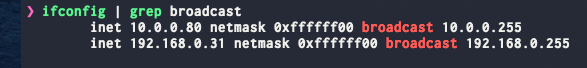
\includegraphics[width=0.5\textwidth]{ifconfig.png}
\caption{First the command 'ifconfig | grep broadcast' identifies the local networks.}\label{ifconfig image}
\end{figure}

\medskip
\subsection*{super user privileges for scanning}
Next I ran a ping scan of both networks to quickly get a list of the hosts. It's likely that you will not get a full list if you do not run this command with super user privileges.
Testing this without sudo resulted in 1 host and 9 hosts respectively. To run ping scans for both networks we used:
\begin{verbatim}
sudo nmap -sn 192.168.0.0/24
sudo nmap -sn 10.0.0.0/24 \end{verbatim}

\medskip

\begin{figure}[H]
\centering
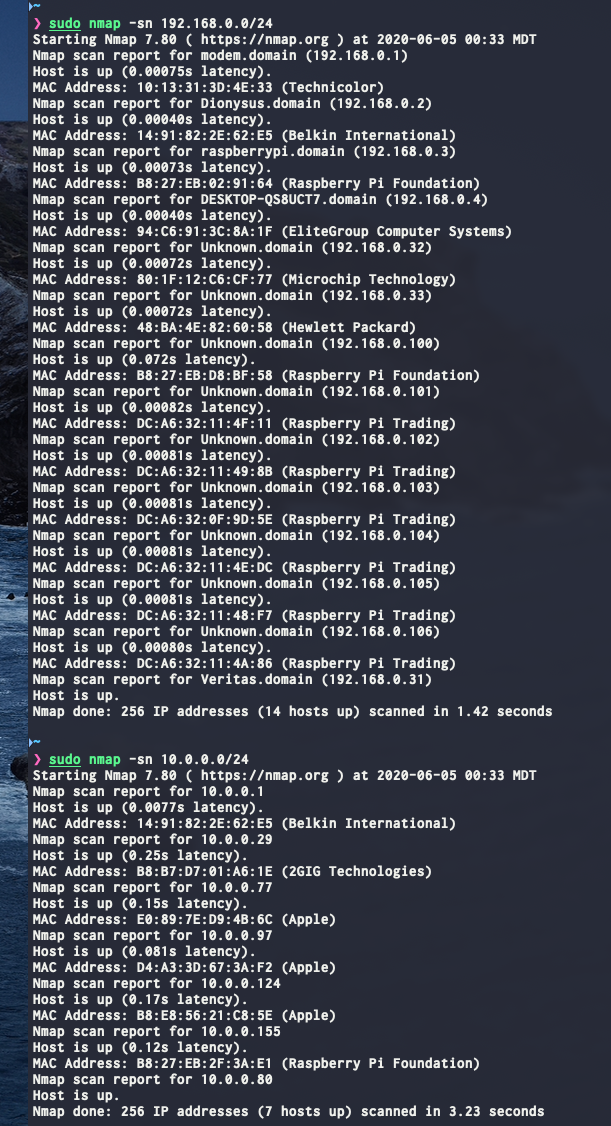
\includegraphics[width=0.5\textwidth]{ping.png}
\caption{Ping scan returning 14 and 7 hosts.}\label{ping image}
\end{figure}
As we can see in \textbf{Figure \ref{ping image}}, the ping scan with sudo returned a list of 14 hosts and 7 hosts respectively. 

\subsection*{Nmap flags for more thorough scans}
After completing the quick and simple ping scan we scanned both networks using nmap with the flag \verb|-A| to initiate an agressive scan. We also included \verb|-v| to increase the 
verbosity of our results and \verb|-T5| to turn the scans speed all the way up. The commands used:
\begin{verbatim}
sudo nmap -T5 -A -v 192.168.0.0/24
sudo nmap -T5 -A -v 10.0.0.0/24\end{verbatim}
At this point it was necessary to create \textbf{Table \ref{local table}} to organize the results and create an overview that could actually be visualized. These 
types of scans return so much information that it demands systematic organization. Zenmap can do a good job of helping with this but it has not been running
well for me on macOS Catalina. Another option which I employed is to use an additional flag when running nmap \verb|-oX 'scan-%T-%D.xml'| which outputs the
scan in xml format named by the date and time. To give some full examples:
\begin{verbatim}
sudo nmap -oX 'scan-%T-%D.xml' -T5 -A -v 192.168.0.0/24
sudo nmap -oX 'scan-%T-%D.xml' -T5 -A -v 10.0.0.0/24\end{verbatim}

\subsection*{monitoring public IP addresses with shodan.io}
Due to the ethical and legal restrictions on scanning the public IP owned by Century Link I used shodan.io to search for my IP and set up a monitor for the address.\cite{shodan}
An easy what to determine your public IP address is with command:
\begin{verbatim}
 curl ifconfig.me
\end{verbatim}

\section*{results}
To begin with, shodan.io allowed us to determine that our router has an open outward facing port running http with authentication.\cite{shodan} \textbf{Figure \ref{shodan image}} 
shows a screen shot from their webservice.

\begin{figure}[H]
\centering
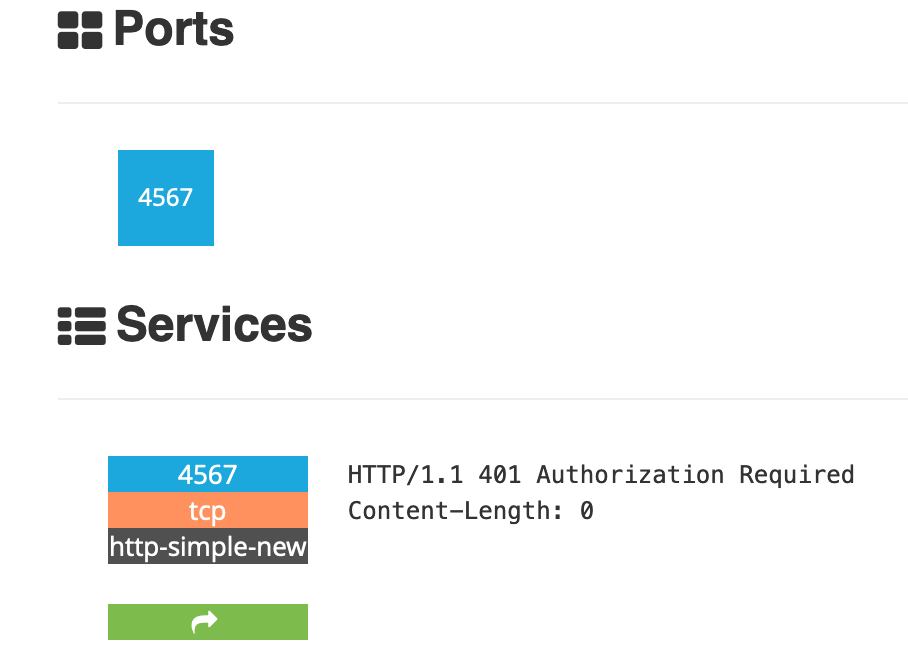
\includegraphics[width=0.5\textwidth]{shodan.png}
\caption{From website https://www.shodan.io/ often called "the most dangerous search engine in the world"}\label{shodan image}
\end{figure}

\subsection*{Compiling all of the findings}
The table below, \textbf{Table \ref{local table}}, is a compilation of all the scans. The aggressive scans discovered more hosts missed by the privileged ping scans.
Immediately some interesting things are visible from the table. First, my HomePod has two IP addresses on the same network. After logging into and checking the router
it appeared that both were running on the 5G wifi. While going through the devices I was familiar with all of the results except for 192.168.0.32 which was running ssh
on port 22. I check the routers DCHP Reservations and found no information there either. The scan did show the mac address \verb|80:1F:12:C6:CF:77| as well as some
additional information. Seen here using a targeting scan of just this device: \verb|sudo nmap -T5 -A 192.168.0.32| 

\begin{figure}[H]
\centering
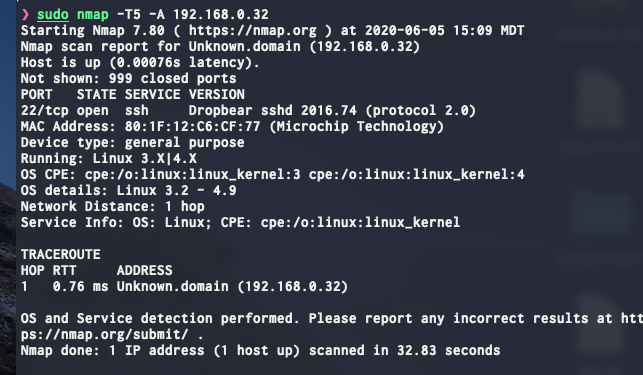
\includegraphics[width=0.5\textwidth]{unknown.png}
\caption{Resulting scan of unfamiliar device}\label{unknown image}
\end{figure}

\begin{table}[H]
  \begin{center}
  \begin{tabular}{ | c | c | c | c | c | c | c | c | } 
  \hline
   & \textbf{Hostname} & \textbf{Device} & \textbf{Purpose} & \textbf{OS} & \textbf{Open} & \textbf{Filtered}  & \textbf{Services}  \\  
   \hline
   \textbf{10.0.0.001} & Dionysus & Router & Gateway & Linux & 53,80,443,10000 & - & ssl,http \\  
   \hline
   \textbf{10.0.0.029}  & HD100 & Webcam & Security & - & 554,49152 & - & rtsp,UPnP \\  
   \hline
   \textbf{10.0.0.077}  & Daemon & HomePod & Music & audioOS & 62078 & 24 dif & wiretap\\  
   \hline
   \textbf{10.0.0.080}  & Veritas & MacLaptop & PC & macOS & 3000 & - & grafana \\  
   \hline
   \textbf{10.0.0.097}  & Daemon & HomePod & Music & audioOS & 6 dif & 100 dif & wiretap \\  
   \hline
   \textbf{10.0.0.124}  & Mercury & Watch & Fit & watchOS & - & 17 dif & wiretap/track \\  
   \hline
   \textbf{10.0.0.155}  & raspberrypi & rpi & dev & Buster & 22 & - & ssh \\  
   \hline
   \textbf{}  &  &  &   &  &  &  & \\  
   \hline
   \textbf{192.168.0.001}  & Century Link & Router & Gateway & Linux & 23,80,433,8085 & - & telnet\\  
   \hline
   \textbf{192.168.0.002}  & Dionysus & Router & Secondary & Linux & All & - & - \\  
   \hline
   \textbf{192.168.0.003}  & raspberrypi & rpi & dev & Buster & 22 & - & ssh \\  
   \hline
   \textbf{192.168.0.004}  & DESKTOP.. & WindowsPC & PC & Windows & - & All & - \\  
   \hline
   \textbf{192.168.0.031} & Veritas & MacLaptop & PC & macOS & 3000 & - & grafana \\
   \hline
   \textbf{192.168.0.032} & Unknown & ? & 80:1f:12:c6:cf:77 & Linux & 22 & - & ssh \\
   \hline
   \textbf{192.168.0.033} & Unknown & HPLaptop & tails & tails live & - & All & - \\  
   \hline
   \textbf{192.168.0.100}  & Ares & rpi & motion & Buster & 22,3389,8081 & - & xrdp,motion \\  
   \hline
   \textbf{192.168.0.101}  & Master & rpi & Kubernetes & Buster & 22,80,443 & - & - \\  
   \hline
   \textbf{192.168.0.102}  & Node1 & rpi & Kubernetes & Buster & 22,80,443 & - & - \\  
   \hline
   \textbf{192.168.0.103}  & Node2 & rpi & Kubernetes & Buster & 22,80,443 & - & - \\  
   \hline
   \textbf{192.168.0.104}  & Node3 & rpi & Kubernetes & Buster & 22,80,443 & - & - \\  
   \hline
   \textbf{192.168.0.105}  & Node4 & rpi & Kubernetes & Buster & 22,80,443 & - & - \\  
   \hline
   \textbf{192.168.0.106}  & Node5 & rpi & Kubernetes & Buster & 22,80,443 & - & - \\  
   \hline
  \end{tabular}
  \caption{Compilation of the results from all scans. Purpose column filled from previous knowledge of the network.}
  \label{local table}
  \end{center}
  \end{table}

\subsection*{identifying the unknown device}
Attempting to connect via ssh to the device confirmed that it was not something I was familiar with. I change all of my ssh
connections to passwordless key based authentication. This has much better security than the password based authentication
running on this device which allowed me to connect and try passwords as well as connect as root to try passwords which 
I regularly disallow.

\subsection*{researching the OUI}
Nmap includes a lookup of the mac addresses OUI, organizationally unique identifier, the first three octets.
\begin{verbatim}
MAC Address: 80:1F:12:C6:CF:77 (Microchip Technology)
\end{verbatim}

\subsection*{binary note}
Note that in the decimal notation representing the last octet of our networking addresses 3 digits are required
whereas here hexidecimal notation is used and only two digits are required. Both of these represent 8 binary digits
and have 256 unique possibilities. Usually indexed at 0 so 0-255 and in the case of networking some addresses are always reserved.
\medskip

The products section of their website at \verb|https://www.microchip.com/| included embedded architecture,
security, smart monitoring and networking devices among others.\cite{microchip} This prompted the question, could my security device
for the lock on my door have started running in unsecure ssh connection on my network as soon as I plugged in the 
ethernet cable?

\subsection*{unplug that device}
Immediately unplugging the device then rescanning confirmed this hypothesis as seen in \textbf{Figure \ref{down image}}.

\begin{figure}[H]
\centering
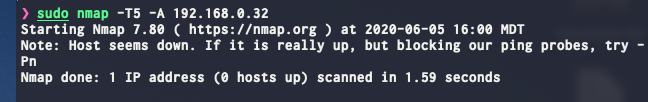
\includegraphics[width=0.5\textwidth]{down.png}
\caption{Rescan after unplugging}\label{down image}
\end{figure}




\section*{conclusions}
The scans and research prompted some further action. To look more closely into the \verb|4567 tram| port open on the router to the internet I enabled telnet and
explored the device. I was curious to see if the port could be closed but didn't find a method. Throughout the research I did find a possible ADSL attack vector 
for the router:\cite{techni}
\begin{verbatim}
  nmap -sS -sV -vv -n -Pn -T5 A.B.C.D -p80 -oG -
\end{verbatim}
This attack was summarized, \verb|using nmap to look for an open port 80 on a huge block of IP addresses|.\cite{techni} 
Article, \verb|The weakest link on the network: exploiting ADSL routers to perform cyber-attacks|, published by the IEEE 
in 2013 discusses their discovery of two 0-day vulnerabilities and expounds the vulnerabilities of ADSL routers.\cite{journal} Of course my conscience of the ethical and legal 
concerns prevented me from attempting any attacks without explicit permission.

\subsection*{the intelligence of smart security devices}
The most concerning finding on my local network was the opreation of the security device which controls my locks and that was mandated for all 
apartment units. Along with a possible network attack vector, I was able to plug and unplug the device because it is not stored in a secure cabinet. I have total 
access to it. All of the devices in my building are the same so if one is compromised every unit is compromised. Likely nationwide a huge number of homes would be 
compromised. Access also gave me the FCC IDs seen in \textbf{Figure \ref{fcc1 image}}.
\begin{figure}[H]
\centering
\includegraphics[width=0.5\textwidth]{fcc1.png}
\caption{The FCC ID's clearly displayed}\label{fcc1 image}
\end{figure}

\subsection*{fcc id}
The FCC ID's listed are \verb|2AAU7-ZB2ZWUS XMR201807EG91NA| and are all matters of public record. The FCC website is pretty terrible to use but using
\verb|www.fcc.io| we can search FCC site with a much better UI. The records tell us that the device has a Quectel Wireless chip for the cellular connection
as well as a Z-Wave module to connect to the devices.\cite{fcc} Leaving the cellular aside the records give us two possible frequencies for the radio communication
to the locks. In \textbf{Figure \ref{radio image}} we can see one of the radio frequencies.\cite{fcc} It is beyond the scope of this paper but a software 
defined radio could be used to capture and analize the signals on that frequency.

\begin{figure}[H]
\centering
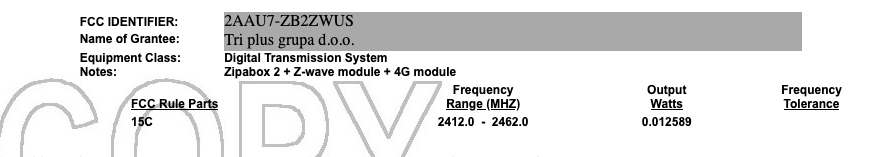
\includegraphics[width=0.5\textwidth]{radio.png}
\caption{Radio frequency}\label{radio image}
\end{figure}

\subsection*{nmap OS fingerprinting}
Many of the devices on my network had operating systems which were unrecognized and nmap asked to submit the fingerprint if the OS is known. I followed the link to try 
and submit the fingerprints but ran into a bug on the Nmap site. There was no section on the submission form for writing what the OS actually was, \textbf{Figure \ref{bug image}}. 
On the site to submit service types there was the section missing from the OS submission page. I signed up to the dev-mailing list, as suggested by the site for bug 
reporting, to try and see if the bug was known.\cite{submit} I also ran into several issues with Zenmap on Catalina from install, to running, to save permissions and with it 
crashing when selecting topology.

\medskip

\subsection*{next steps}
In addition to the further avenues for research within the network, next steps would include more testing on these issues and bug reporting to nmap dev-list and issue
trackers.

\begin{figure}[H]
\centering
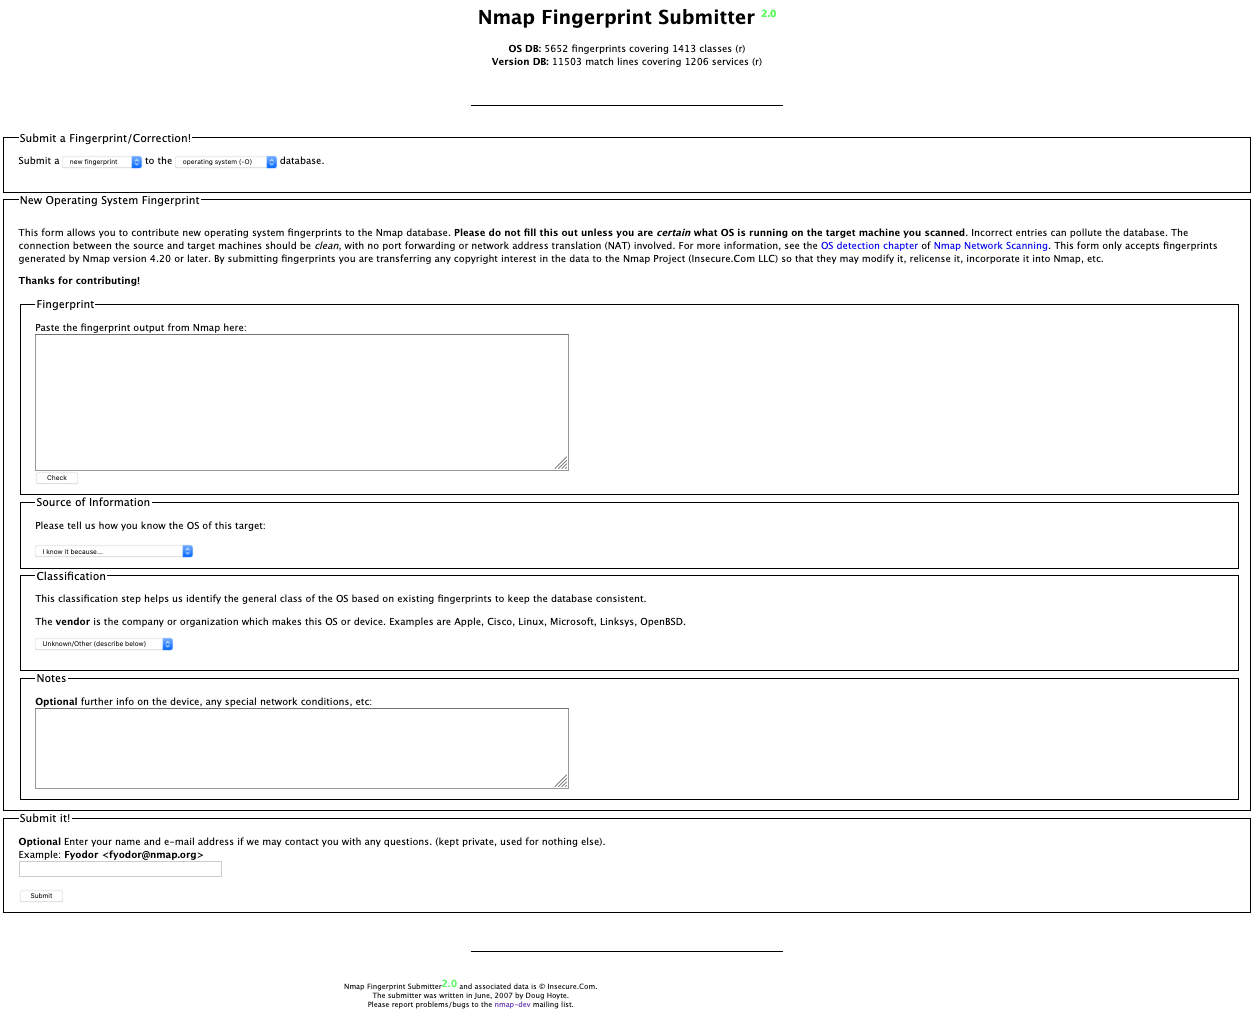
\includegraphics[width=0.75\textwidth]{bug.png}
\caption{Nmap OS fingerprint submission page missing OS name category}\label{bug image}
\end{figure}

\begin{thebibliography}{9} 

\bibitem{journal} Stasinopoulos, Ntantogian and  Xenakis(2013) The weakest link on the network: Exploiting ADSL routers to perform cyber-attacks, \textit{IEEE International Symposium on Signal Processing and Information Technology} 000135-000139. \textit {https://doi.org/10.1109/ISSPIT.2013.6781868}

\bibitem{shodan} The search engine for The Internet of Things, \textit{https://www.shodan.io/} (accessed June 2020)

\bibitem{techni} Technicolor C2100T, \textit{https://charlesreid1.com/wiki/Technicolor\_C2100T} (accessed June 2020)

\bibitem{microchip} Microchip Technology Inc, \textit{https://www.microchip.com/} (accessed June 2020)

\bibitem{fcc} Federal Communications Commission, \textit{https://www.fcc.gov/} (accessed June 2020)

\bibitem{submit} Nmap Fingerprint Submitter, \textit{https://nmap.org/cgi-bin/submit.cgi?new-os} (accessed June 2020)

\end{thebibliography}


\section*{reflection}
There were some changes I made to the configuration of my network on the basis of this paper. I realized that I should be turning 
grafana off when I am not using it until I have it setup with production level safety. I decided that my smart device was better off 
having less connectivity and that I would not be plugging it into my local network. It was interesting to check what returned from the 
tails during network scans, which was nothing at all and a mac address which changed on every boot. It was also suprising to see how
many services actively run on my HomePod and my appleWatch as well as the HomePod using two IP addresses. I hadn't explored the telnet
connection to my CenturyLink device before either and it was a good learning experience. It was interesting to see how different the telnet
interfaces are between devices. I'd been meaning to check the protocols on the smart security device and so was glad to get a chance. I 
think the current version of Z-wave is relatively secure but found some talk about downgrade attacks forcing devices to use older
versions. I also used this as an opportunity to try using LaTeX for the first time, which I borderline came to regret as I didn't realize
before hand that there is come complexity to it. I especially struggled when towards the end I was getting tired and it was time to figure 
out the formatting for the bibliography and citations. Also if I had more time I would have looked more closely into exactly what was and 
wasn't returned from the different nmap scans including UDP scans and see if I could find more information locally using options for firewall 
evasion and IDS evasion.

\end{document}
